\documentclass[14pt,a4paper]{extarticle}

\usepackage{fontspec}
\setmainfont{Times New Roman}
\setmonofont{Courier New}[Scale=0.9]
\newfontfamily\arialfont{Arial}

\usepackage[russian]{babel}
\usepackage{amsmath}
\usepackage{amssymb}
\usepackage{amsfonts}
\usepackage{multirow}

\usepackage{geometry}
\geometry{left=3cm,right=1.5cm,top=2cm,bottom=2cm}

\usepackage{setspace}
\onehalfspacing
\setlength{\parindent}{1.25cm}

\usepackage{ragged2e}
\emergencystretch=1.5em

\usepackage{titlesec}
\titleformat{\section}
  {\arialfont\bfseries\fontsize{14pt}{16pt}\selectfont\centering}
  {\thesection} 
  {1em} 
  {} 
\titlespacing*{\section}{0pt}{1.5ex plus 1ex minus .2ex}{1.5ex plus .2ex}

\titleformat{name=\section,numberless}
  {\arialfont\bfseries\fontsize{14pt}{16pt}\selectfont\centering}
  {}
  {0pt}
  {}

\titleformat{\subsection}
  {\arialfont\bfseries\fontsize{14pt}{16pt}\selectfont}
  {\thesubsection}
  {1em}
  {}
\titlespacing*{\subsection}{0pt}{1.3ex plus .2ex}{1ex plus .2ex}

\usepackage{graphicx}
\usepackage{tabularx}
\usepackage{booktabs}
\usepackage{float}
\usepackage{caption}

\usepackage{listings}
\lstset{
    basicstyle=\ttfamily\fontsize{14pt}{16pt}\selectfont,
    breaklines=true,
    frame=none,
    showstringspaces=false,
    tabsize=4,
    extendedchars=true,
    literate={а}{{\cyrchar\CYRA}}1 {б}{{\cyrchar\CYRB}}1 {в}{{\cyrchar\CYRV}}1 {г}{{\cyrchar\CYRG}}1 {д}{{\cyrchar\CYRD}}1 {е}{{\cyrchar\CYRE}}1 {ё}{{\cyrchar\CYRYO}}1 {ж}{{\cyrchar\CYRZH}}1 {з}{{\cyrchar\CYRZ}}1 {и}{{\cyrchar\CYRI}}1 {й}{{\cyrchar\CYRISHRT}}1 {к}{{\cyrchar\CYRK}}1 {л}{{\cyrchar\CYRL}}1 {м}{{\cyrchar\CYRM}}1 {н}{{\cyrchar\CYRN}}1 {о}{{\cyrchar\CYRO}}1 {п}{{\cyrchar\CYRP}}1 {р}{{\cyrchar\CYRR}}1 {с}{{\cyrchar\CYRS}}1 {т}{{\cyrchar\CYRT}}1 {у}{{\cyrchar\CYRU}}1 {ф}{{\cyrchar\CYRF}}1 {х}{{\cyrchar\CYRH}}1 {ц}{{\cyrchar\CYRC}}1 {ч}{{\cyrchar\CYRCH}}1 {ш}{{\cyrchar\CYRSH}}1 {щ}{{\cyrchar\CYRSHCH}}1 {ъ}{{\cyrchar\CYRHRDSN}}1 {ы}{{\cyrchar\CYRERY}}1 {ь}{{\cyrchar\CYRSFTSN}}1 {э}{{\cyrchar\CYREREV}}1 {ю}{{\cyrchar\CYRYU}}1 {я}{{\cyrchar\CYRYA}}1
}
\usepackage{tocloft}
\usepackage[unicode, colorlinks=true, linkcolor=black, urlcolor=black, citecolor=black]{hyperref}

\addto\captionsrussian{\renewcommand{\contentsname}{СОДЕРЖАНИЕ}}

\renewcommand{\cfttoctitlefont}{\hspace*{\fill}\arialfont\bfseries\fontsize{14pt}{16pt}\selectfont}
\renewcommand{\cftaftertoctitle}{\hspace*{\fill}}

\renewcommand{\cftsecfont}{\mdseries\normalfont}
\renewcommand{\cftsecpagefont}{\mdseries\normalfont}
\renewcommand{\cftsubsecfont}{\mdseries\normalfont}
\renewcommand{\cftsubsecpagefont}{\mdseries\normalfont}

\renewcommand{\cftsecleader}{\cftdotfill{\cftdotsep}}
\renewcommand{\cftsubsecleader}{\cftdotfill{\cftdotsep}}

\counterwithin{figure}{section}
\counterwithin{table}{section}

\setlength{\cftsecindent}{0em}
\setlength{\cftsubsecindent}{0em}
\setlength{\cftbeforesecskip}{0pt}    
\setlength{\cftbeforesubsecskip}{0pt} 
\usepackage{pgfplots}
\pgfplotsset{compat=1.18}
\usepgfplotslibrary{groupplots}

\begin{document}

\justifying

\begin{titlepage}
    \fontsize{14pt}{16pt}\selectfont
    
    \begin{center}
        \textbf{МИНОБРНАУКИ РОССИИ} \\
        \textbf{САНКТ-ПЕТЕРБУРГСКИЙ ГОСУДАРСТВЕННЫЙ} \\
        \textbf{ЭЛЕКТРОТЕХНИЧЕСКИЙ УНИВЕРСИТЕТ} \\
        \textbf{«ЛЭТИ» ИМ. В.И. УЛЬЯНОВА (ЛЕНИНА)} \\
        \textbf{Кафедра алгоритмической математики}
    \end{center}

    \vspace{3cm}

       \begin{center}
        \begin{spacing}{1.5}
            \textbf{ОТЧЕТ} \\
            \textbf{по лабораторной работе №1} \\
            \textbf{по дисциплине «Криптография и защита информации»} \\
            \textbf{Тема: Экспериментальное определение количества раундов} \\
            \textbf{вероятностного алгоритма} \\
            \textbf{Вариант: Поиск числа с заданным показателем по простому} \\
            \textbf{модулю с использованием теста простоты Соловея – Штрассена}
        \end{spacing}
    \end{center}
    \vfill

    \noindent
    \makebox[5cm][l]{Студент гр. 3385} \hfill \underline{\hspace{6cm}} \hspace{0.3cm} Баринов М.А. \\[0.3cm]
    \noindent
    \makebox[5cm][l]{Студент гр. 3385} \hfill \underline{\hspace{6cm}} \hspace{0.3cm} Комаренко Т.А.

    \vspace{1cm}

    \noindent
    \begin{minipage}[c]{0.70\textwidth}
        \renewcommand{\arraystretch}{1.2}
        \begin{tabularx}{\textwidth}{|>{\centering\arraybackslash}X|>{\centering\arraybackslash}X|>{\centering\arraybackslash}X|>{\centering\arraybackslash}X|>{\centering\arraybackslash}X|}
            \hline
            {\fontsize{10pt}{12pt}\selectfont Теория} & 
            {\fontsize{10pt}{12pt}\selectfont Реализация} & 
            {\fontsize{10pt}{12pt}\selectfont Эксперимент} & 
            {\fontsize{10pt}{12pt}\selectfont Оформление} & 
            {\fontsize{10pt}{12pt}\selectfont Защита} \\
            \hline
            \rule{0pt}{1.0cm} & & & & \\ 
            \hline
        \end{tabularx}
    \end{minipage}
    \hfill
    \begin{minipage}[c]{0.28\textwidth}
        \begin{tabular}{@{}l@{}}
            защищено \underline{\hspace{0.4cm}} . \underline{\hspace{0.4cm}} . \underline{\hspace{0.8cm}} \\[0.1cm] 
            с \underline{\hspace{2.2cm}} попытки \\[0.1cm] 
            с оценкой \underline{\hspace{2.2cm}}
        \end{tabular}
    \end{minipage}

    \vspace{1cm}

    \noindent
    \makebox[5cm][l]{Преподаватель} \hfill \underline{\hspace{6cm}} \hspace{0.3cm} Абросимов И.К.

    \vfill
    \begin{center}
        Санкт-Петербург \\
        2026
    \end{center}
\end{titlepage}

\newpage
\section*{ЗАДАНИЕ НА ЛАБОРАТОРНУЮ РАБОТУ}

\begin{spacing}{1.5} 

\noindent Студенты Баринов М. А., Комаренко Т. А. группы 3385 \\
Тема работы: экспериментальное исследование количества раундов вероятностного алгоритма поиска числа с заданным мультипликативным порядком по простому модулю с использованием теста простоты Соловея–Штрассена.

\vspace{0.5cm}
\noindent \textbf{Задание на лабораторную работу:}
\begin{enumerate}
    \item Реализовать на языке C++ с использованием длинной целочисленной арифметики алгоритм поиска числа с заданным мультипликативным порядком по простому модулю, а также тест простоты Соловея–Штрассена. При реализации разрешается использовать только операции ввода-вывода, сложения, вычитания, сравнения, сдвига и побитовые операции (общее деление с остатком запрещено).
    \item Провести экспериментальную оценку количества раундов вероятностного алгоритма.
\end{enumerate}

\noindent Содержание пояснительной записки: разделы «СОДЕРЖАНИЕ», «ТЕОРЕТИЧЕСКОЕ ВВЕДЕНИЕ» с подразделами «Описание исследуемого алгоритма» и «Методика экспериментального исследования», «РЕШЕНИЕ ПОСТАВЛЕННОЙ ЗАДАЧИ» с подразделами «Реализация исследуемого алгоритма», «Тестирование реализации алгоритма», «Проведение эксперимента» и «Обработка результатов эксперимента», «ЗАКЛЮЧЕНИЕ», «СПИСОК ИСПОЛЬЗУЕМЫХ ИСТОЧНИКОВ».

\noindent Предполагаемый объем пояснительной записки: не менее 25 страниц.

\vspace{1.5cm}
\newpage
\noindent Дата выдачи задания: 15.10.2026 \\
Дата сдачи пояснительной записки: 03.11.2026 \\
Задание получил \underline{\hspace{3cm}} Баринов М.А. \\
Задание получил \underline{\hspace{3cm}} Комаренко Т.А. \\
Задание выдал \underline{\hspace{3cm}} Абросимов И.К.

\end{spacing}

\newpage
\makeatletter
\renewcommand{\numberline}[1]{}
\makeatother

\tableofcontents
\newpage

\makeatletter
\renewcommand{\numberline}[1]{\hb@xt@\@tempdima{\hss#1\enspace}}
\makeatother
\makeatletter
\renewcommand{\numberline}[1]{\hb@xt@\@tempdima{\hss#1\enspace}}
\makeatother

\makeatletter
\renewcommand{\numberline}[1]{\hb@xt@\@tempdima{\hss#1\enspace}}
\makeatother

\section{ТЕОРЕТИЧЕСКОЕ ВВЕДЕНИЕ}
\begin{spacing}{1.5} 
Цель работы: экспериментальное определение количества раундов вероятностного алгоритма.

\subsection{Описание исследуемого алгоритма}
\textbf{Определение.} Пусть \(m\) — натуральное число, \(a\) — целое число, взаимно простое с \(m\). Мультипликативным порядком числа \(a\) по модулю \(m\) называется наименьшее натуральное \(n\), такое что
\begin{equation}\tag{1.1}
    a^n \equiv 1 \pmod m,
\end{equation}
обозначаемое \(P_m(a)\).

\textbf{Определение.} Функция Кармайкла – функция, определяемая при известном разложении аргумента на простые множители формулой

\begin{equation}\tag{1.2}
    \lambda(m) = \left[
        \begin{array}{ll}
        L(m), & m = 2^{d_0'} \cdot m', \\
        M(2^{d_0}, L(m')), & m = 2^{d_0+2} \cdot m',
        \end{array}
    \right.
\end{equation}
где \(d_0' \in \overline{0,2}\), \(d_0 \in \mathbb{N}\), \(m' \in (\mathbb{N} \setminus 2\mathbb{N})\).

\textbf{Утверждение} (Совпадение значений функций Эйлера и функции Кармайкла). Если \(m\) равно 2 или 4 или натуральной степени нечетного простого числа или удвоенной натуральной степени нечетного простого числа, то значения функции Эйлера и функции Кармайкла в точке \(m\) равны, т.е.
\begin{equation}\tag{1.3}
    m \in (\{2, 4\} \cup P \cup (2P)) \Rightarrow \phi(m) = \lambda(m),
\end{equation}
где \(P = \{p^n \mid p \in \mathbb{P}'_{\mathbb{N}}, n \in \mathbb{N}\}\), \(\mathbb{P}'_{\mathbb{N}} = \mathbb{P}_{\mathbb{N}} \setminus \{2\}\).

Поиск значения показателя по модулю можно осуществлять согласно следующему \textbf{утверждению} (множество возможных значений показателя по модулю). Множество возможных значений показателя по модулю \(m\) принадлежит натуральным делителям \(\lambda(m)\), т. е.
\begin{equation}\tag{1.4}
    P_m(a) \in d(\lambda(m)),
\end{equation}
где \(a \perp m\).

Значение мультипликативного порядка по модулю от натуральной степени числа связано с значением порядка от основания этой степени согласно \textbf{утверждению} (мультипликативный порядок степени натурального числа):
\begin{equation}\tag{1.5}
    \gamma = P_m(a) \Rightarrow P_m(a^b) = \frac{\gamma}{D(\gamma, b)},
\end{equation}
где \(D(\gamma, b)\) - наибольший общий делитель чисел \(\gamma\) и \(b\).

Значение мультипликативного порядка по модулю \(m\) натуральной степени с показателем, равным отношению значения \(\lambda(m)\) и ее некоторого делителя \(q\), ограничено согласно \textbf{утверждению} (оценка сверху значения мультипликативного порядка):
\begin{equation}\tag{1.6}
    a^{\frac{\lambda(m)}{q}} \not\equiv 1 \pmod m \Rightarrow P_m(a^{\frac{\lambda(m)}{q}}) \leq q.
\end{equation}

Для тестирования числа на соответствие заданному мультипликативному порядку применяется следующее \textbf{утверждение}. Если \(b \equiv a^{\frac{\lambda(m)}{q}} \not\equiv 1 \pmod m\) и при всех простых делителях \(e\) числа \(q\) справедливы утверждения \(b^{\frac{q}{e}} \not\equiv 1 \pmod m\), то число \(b\) имеет порядок \(q\) по модулю \(m\), т. е.
\begin{equation}\tag{1.7}
    \forall e \in (d(q) \cap \mathbb{P}_N) \quad b^{\frac{q}{e}} \not\equiv 1 \pmod m \Rightarrow P_m(b) = q,
\end{equation}
Где \(b \equiv a^{\frac{\lambda(m)}{q}} \not\equiv 0 \pmod m\), \(a\) - произвольное число, взаимно простое с \(m\) и несравнимое с 1 по модулю \(m\).

\textbf{Вероятностный алгоритм поиска числа с заданным показателем.} Раунд вероятностного алгоритма поиска числа с заданным мультипликативным порядком \(q \mid \lambda(m)\) по модулю \(m\) состоит из следующих шагов:
\begin{enumerate}
    \item Выбрать случайное число \(a\) так, что \(1 \le a \le m-1\);
    \item Вычислить \(D(a, m)\). Если \(D(a, m) > 1\), то вернуться на шаг 1;
    \item Вычислить \(b \equiv a^{\frac{\lambda(m)}{q}} \pmod m\). Если \(b = 1\), то вернуться на шаг 1;
    \item Для всех простых делителей \(\{q_j, j \in \overline{1, n}\}\) числа \(q\) вычислить \(c_j \equiv b^{\frac{q}{q_j}} \pmod m\). Если очередное \(c_j = 1\), то вернуться на шаг 1.
\end{enumerate}

Результат: число \(b\) такое, что \(P_m(b) = q\).

Эффективность этого алгоритма основывается на следующем утверждении (вероятность успеха при поиске числа с заданным показателем по простому модулю). При случайном выборе \(1 \le a \le m-1\), где \(m\) - простое число, вероятность того, что \(b \equiv a^{\frac{m-1}{q}} \pmod m\) будет иметь показатель \(q\) по модулю \(m\), равно \(\frac{\phi(q)}{q}\). 

Тест простоты Соловея-Штрассена основан на утверждении: если \(m\) – нечетное составное число, то количество целых чисел \(a\), взаимно простых с \(m\) и меньших \(m\) удовлетворяющих сравнению
\begin{equation}\tag{1.8}
    a^{\frac{m-1}{2}} \equiv \left(\frac{a}{m}\right) \pmod m,
\end{equation}
не превосходит \(\left\lfloor \frac{m}{2} \right\rfloor\). Здесь \(\left(\frac{a}{m}\right)\) - символ Якоби. Таким образом, если для некоторого \(a\) имеет место утверждение \(a^{\frac{m-1}{2}} \not\equiv \left(\frac{a}{m}\right) \pmod m\), то \(m\) - заведомо составное число, иначе \(a\) - называют свидетелем простоты числа \(m\).

Доказательство всех утверждений приведено в разделе «ПРИЛОЖЕНИЕ А. Доказательства используемых утверждений».

\subsection{Методика экспериментального исследования}
Распределение затрат — зависимость количества \(N(R)\) запусков алгоритма, для которых потребовалось ровно \(R\) раундов, от количества раундов.

Графиком распределения затрат является гистограмма: по горизонтальной оси откладываются возможные значения количества раундов, по вертикальной — количество запусков, при которых алгоритм завершился за данное количество раундов.

Если количество возможных входных данных не слишком велико, используется полный перебор; в противном случае — метод Монте-Карло:
\begin{enumerate}
    \item Зафиксировать количество \(n\) испытаний (например, \(n = 1000\));
    \item Для каждого испытания выполнить алгоритм, замерив количество \(R_j\) раундов;
    \item Построить гистограмму распределения затрат: определить минимум и максимум множества \(\{R_j\}\), при необходимости объединить значения в интервалы;
    \item Найти среднюю, медианную и модальную сложности (в раундах), а также оценить, насколько полученное распределение близко к \(p = \frac{\phi(q)}{q}\).
\end{enumerate}

Пусть \(R_i, i \in \overline{1, n}\) - количество раундов в \(i\)-ом испытании. Среднее, медианное и модальное значения вычисляются по формулам:
\begin{equation}\tag{1.9}
    R_{avg} = \frac{1}{n} \sum_{i=1}^{n} R_i,
\end{equation}
\begin{equation}\tag{1.10}
    R_{med} = \operatorname{med}\{R_i, i \in \overline{1, n}\},
\end{equation}
\begin{equation}\tag{1.11}
    R_{\text{mode}} = \operatorname{mode}\{R_i, i \in \overline{1, n}\},
\end{equation}

Среднее значение показывает, сколько раундов в среднем требуется алгоритму при случайном выборе \(a\). Медиана делит отсортированное множество замеров на две равные части. Мода — наиболее часто встречающееся количество раундов.

Теоретическое среднее равно \(\frac{q}{\phi(q)}\). Сравнение эмпирического среднего с теоретическим позволяет проверить корректность реализации и справедливость вероятностной оценки.
\end{spacing}

\newpage
\section{РЕШЕНИЕ ПОСТАВЛЕННОЙ ЗАДАЧИ}
\begin{spacing}{1.5} 
\subsection{Реализация исследуемого алгоритма}
Согласно заданию, модуль \(m\) может быть достаточно большим, поэтому при реализации используется библиотека длинной целочисленной арифметики GMP (класс \texttt{mpz\_class}). Главным ограничением задания является запрет на использование операций общего деления с остатком / и \%. Перечень используемых операций и функций приведен в разделе «ПРИЛОЖЕНИЕ Б. Используемые функции».

Поскольку по условию задачи модуль \(m\) является простым числом, а \(q\) и \(q_j\) меньше \(m\), вместо деления используется малая теорема Ферма. Согласно ей, обратный элемент по модулю \(m\) вычисляется как \(q^{-1} \equiv q^{m-2} \pmod m\).
Тогда
\begin{equation}\tag{2.1}
    c \equiv \frac{\lambda(m)}{q} \equiv \frac{m-1}{q} \equiv (m-1) \cdot q^{m-2} \pmod m
\end{equation}

Аналогично вычисляются и показатели для проверки делителей:
\begin{equation}\tag{2.2}
    \frac{q}{q_j} \equiv q \cdot q_j^{m-2} \pmod m
\end{equation}

Для реализации умножения и возведения в степень по модулю без использования деления применяются алгоритмы, основанные на сдвигах и сложениях. Функция \texttt{mul\_mod} реализует алгоритм удвоения сложения, а \texttt{pow\_mod} — бинарное возведение в степень. Для нахождения НОД используется бинарный алгоритм Штейна (\texttt{gcd}), а для символа Якоби — бинарный алгоритм (\texttt{jacobi}), которые также не используют деление с остатком в общем виде.

\begin{table}[H]
\caption{Переменные, используемые для реализации алгоритма}
\begin{tabularx}{\textwidth}{|l|X|}
\hline
\textbf{Название} & \textbf{Описание} \\
\hline
    \texttt{c} & показатель степени $\frac{m-1}{q} \pmod m$, вычисленный через обратный элемент \\
\hline
    \texttt{exponents} & вектор показателей $\frac{q}{q_j} \pmod m$ для всех простых делителей $q$ \\
\hline
\texttt{a} & случайно выбранное основание в диапазоне [1, m - 1]; затем перезаписывается значением $a^c \pmod m$, которое проверяется на соответствие порядку q \\
\hline
\texttt{ok} & логический флаг: $true$, если для текущего значения a выполнены все проверки порядка \\
\hline
\end{tabularx}
\end{table}

\begin{table}[H]
\caption{Структуры, используемые для реализации алгоритма}
\begin{tabularx}{\textwidth}{|l|X|}
\hline
\textbf{Название} & \textbf{Описание} \\
\hline
\texttt{OrderResult} & структура, хранящая число x, показатель которого по модулю равен q, и номер раунда round вероятностного алгоритма, за который это число было найдено (по умолчанию -1). \\
\hline
\end{tabularx}
\end{table}

Реализованная функция:
\begin{lstlisting}[language=C++]
OrderResult find_element_with_order(
    const mpz_class& q, 
    const std::vector<mpz_class>& qd, 
    const mpz_class& m, 
    gmp_randclass& rng, 
    int k) 
{
    OrderResult res;
    
    if (m <= 1)
        throw std::invalid_argument("m must be > 1");
    if (q <= 0)
        throw std::invalid_argument("q must be positive");
    if (gcd(q, m - 1) != q)
        throw std::invalid_argument("q must divide m-1");
    if (!util::solovay_strassen(m, 40, rng))
        throw std::invalid_argument("m must be prime");

    if (q == 1) {
        res.x = 1;
        res.round = 0;
        return res;
    }

    const mpz_class c = mul_mod(m - 1, pow_mod(q, m - 2, m), m);

    std::vector<mpz_class> exponents(qd.size());
    for (std::size_t i = 0; i < qd.size(); ++i)
        exponents[i] = mul_mod(q, pow_mod(qd[i], m - 2, m), m);

    for (std::size_t i = 1; i <= k; ++i) {
        std::vector<mpz_class> exponents(qd.size());
        for (std::size_t i = 0; i < qd.size(); ++i)
            exponents[i] = mul_mod(q, pow_mod(qd[i], m - 2, m), m);
        
        mpz_class a = rng.get_z_range(m - 1) + 1;
        a = pow_mod(a, c, m);
        if (a == 1)
            continue;
        
        bool ok = std::none_of(exponents.begin(), exponents.end(),
            [&] (const mpz_class& e) { return pow_mod(a, e, m) == 1; });
        
        if (!ok)
            continue;
        
        res.x = a;
        res.round = i;
        return res;
    }
    
    res.x = mpz_class(-1);
    res.round = -1;
    return res;
}
\end{lstlisting}

\subsection{Тестирование реализации алгоритма}
Для тестирования реализации использовался фреймворк Google test (gtest). Поскольку исследуемый алгоритм является вероятностным, заранее предсказать возвращаемое значение невозможно. Поэтому тесты проверяют свойство (1.7).

Для проведения тестирования на случайных входных данных разработаны вспомогательные функции:
\begin{enumerate}
    \item Генерация случайного простого числа. Генерируется случайное число \(p\) заданной битовой длины, у которого принудительно устанавливаются старший и младший бит в 1. Затем число проверяется тестом простоты Соловея-Штрассена с 40 раундами.
    \item Генерация множества \(q\) из маленьких простых. Выбираются \(k\) случайных простых из набора \(\{3, 5, 7, 11, \dots, 41\}\), после чего вычисляется их произведение \(q\). Это позволяет управлять структурой \(q\) и вероятностью успеха \(p = \frac{\phi(q)}{q}\).
    \item Генерация простого модуля специального вида. Вычисляется \(m = 2 \cdot q \cdot R + 1\), где \(R\) — простое. Если битовая длина \(m\) совпадает с заданной и \(m\) проходит тест на простоту, модуль принимается, а \(q\) и \(R\) являются делителями \(m - 1\).
\end{enumerate}

Для проверки возвращаемого числа на соответствие заданному порядку была разработана функция \texttt{assert\_valid\_order}, которая проверяет свойство (1.7).
\begin{lstlisting}[language=C++]
void assert_valid_order(const mpz_class& x, const mpz_class& q,
\end{lstlisting}

\begin{lstlisting}[language=C++]
const std::vector<mpz_class>& qd, const mpz_class& m) {
    EXPECT_GE(x, 1);
    EXPECT_LT(x, m);
    mpz_class pow_q = modarith::pow_mod(x, q, m);
    EXPECT_EQ(pow_q, 1) << "Failed: x^q != 1 (mod m)";
    for (const auto& d : qd) {
        mpz_class exp = modarith::mul_mod(q, modarith::pow_mod(d, m - 2, m), m);
        EXPECT_NE(modarith::pow_mod(x, exp, m), 1)
            << "Failed: order is smaller than q (divisor " << d << ")";
    }
}
\end{lstlisting}

Тестирование на граничных случаях
\begin{table}[H]
\caption{Граничные значения для проверки функции find\_element\_with\_order.}
\begin{tabularx}{\textwidth}{|c|c|c|X|c|}
\hline
\textbf{Номер теста} & \textbf{m} & \textbf{q} & \textbf{простые делители q} & \textbf{Ожидаемый результат} \\
\hline
1 & 1 & 2 & \{2\} & Исключение \\
\hline
2 & 7 & 0 & \(\emptyset\) & Исключение \\
\hline
2. & 7 & -2 & \(\emptyset\) & Исключение \\
\hline
\end{tabularx}
\end{table}

Тестирование на фиксированных значениях
\begin{table}[H]
\caption{Фиксированные тесты для проверки функции find\_element\_with\_order.}
\begin{tabularx}{\textwidth}{|c|c|c|X|}
\hline
\textbf{Номер теста} & \textbf{m} & \textbf{q} & \textbf{простые делители q} \\
\hline
1 & 7 & 2 & \{2\} \\
\hline
2 & 7 & 3 & \{3\} \\
\hline
3 & 7 & 6 & \{2, 3\} \\
\hline
4 & 11 & 5 & \{5\} \\
\hline
5 & 13 & 4 & \{2\} \\
\hline
6 & 101 & 20 & \{2, 5\} \\
\hline
\end{tabularx}
\end{table}

Также было проведено стресс-тестирование на 64-битных модулях, состоящее из 1000 случайно сгенерированных тестов по правилам, описанным выше. Все 1000 тестов были успешно пройдены.

\subsection{Проведение эксперимента}
Эксперимент проводился по методике, описанной в разделе 1.2. Зафиксированы параметры:
\[ P_{target} = 0.95 \text{ — целевая вероятность успеха;} \]
\[ M = 1000 \text{ — число запусков алгоритма для каждой конфигурации;} \]
\[ bits = 64 \text{ — размер модуля m в битах.} \]

Для исследования зависимости вероятности успеха от структуры \(q\) (а не от размера модуля) в эксперименте варьируется число простых делителей \(q\). Модуль \(m\) генерировался как \(m = 2 \cdot q \cdot R + 1\), где \(R\) — простое, \(m\) — простое. Это гарантирует \(q \mid (m-1)\) и известное разложение \(m-1 = 2 \cdot q \cdot R\).

Для каждого \(k\) от 1 до 8 рассмотрено 5 независимых конфигураций \(q\) (каждая — произведение \(k\) случайно выбранных простых из \(\{3, 5, 7, 11, \dots, 41\}\)) и соответствующий модуль \(m\). Итого 40 конфигураций.

Для каждой пары \((m, q)\) вычислено минимальное число раундов \(N\), при котором \(1 - (1-p)^N > P_{target}\), где \(p = \frac{\phi(q)}{q}\). Алгоритм \texttt{find\_element\_with\_order} запускался \(M = 1000\) раз с лимитом \(N_{max} = 50\) раундов (запас, чтобы не обрезать хвост распределения).

Фиксировались:
\begin{enumerate}
    \item факт успеха (найден \(x\) с \(P_m(x) = q\));
    \item номер раунда \(R\), на котором найден ответ (для гистограммы);
    \item число успехов \(a\), по которому вычислена \(P_{obs} = \frac{a}{M}\);
    \item среднее число раундов \(R_{avg}\) по успешным запускам.
\end{enumerate}

Данные сохранены в \texttt{summary.csv} (по строке на конфигурацию: \(k, trial, q, p_{theor}, N, P_{actual}, P_{obs}, R_{avg}\)) и \texttt{rounds.csv} (гистограмма \(N(R)\)). Общее число запусков алгоритма: \(40 \cdot 1000 = 40000\).

\subsection{Обработка результатов эксперимента}
По экспериментальным данным (раздел 2.3) построены три группы графиков, соответствующие методике, описанной в разделе 1.2: гистограмма распределения затрат \(N(R)\), средняя/медианная/модальная сложности и оценка близости к теоретическому геометрическому распределению.

\textbf{Гистограмма распределения затрат}

\begin{figure}[H]
    \centering
    \makebox[\textwidth][c]{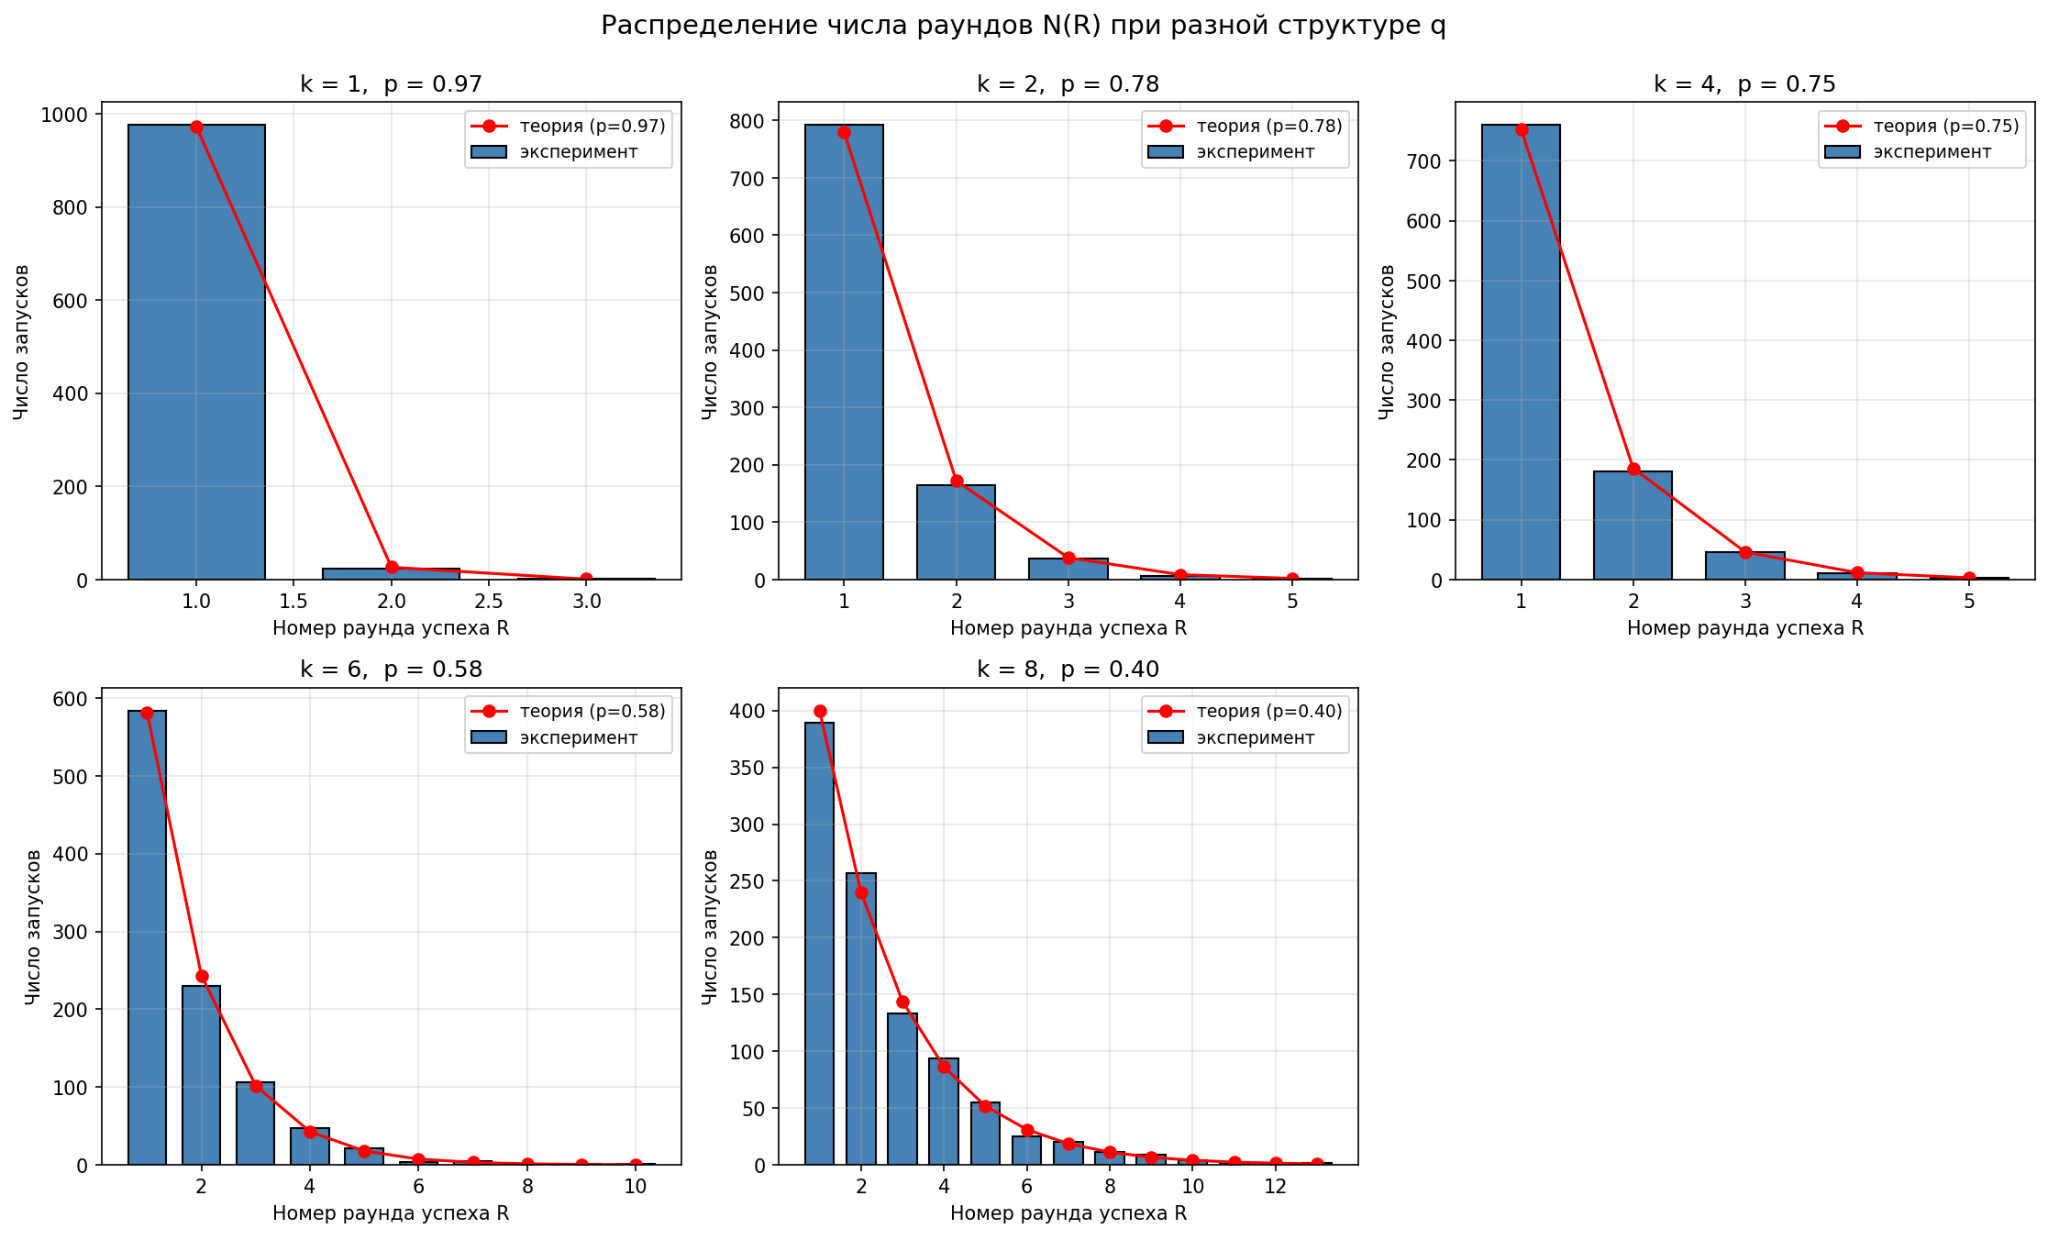
\includegraphics[width=1.15\textwidth]{image/2_1.png}}
    \caption{Распределение числа раундов N(R) для различных k (M = 1000)}
\end{figure}

Из рисунка 2.1 видно, что экспериментальные столбцы во всех конфигурациях совпадают с теоретической кривой. При \(k = 1\) (\(p \approx 0.97\)) распределение резко спадает — большинство запусков находят ответ с 1–2 попыток. С ростом \(k\) (\(p\) уменьшается до 0.40 при \(k = 8\)) распределение становится положе: хвост растягивается на 5–6 раундов. Форма распределения остаётся геометрической при любом \(p\), меняется лишь её параметр.

\textbf{Средняя, медианная и модальная сложности}

\begin{figure}[H]
    \centering
    \makebox[\textwidth][c]{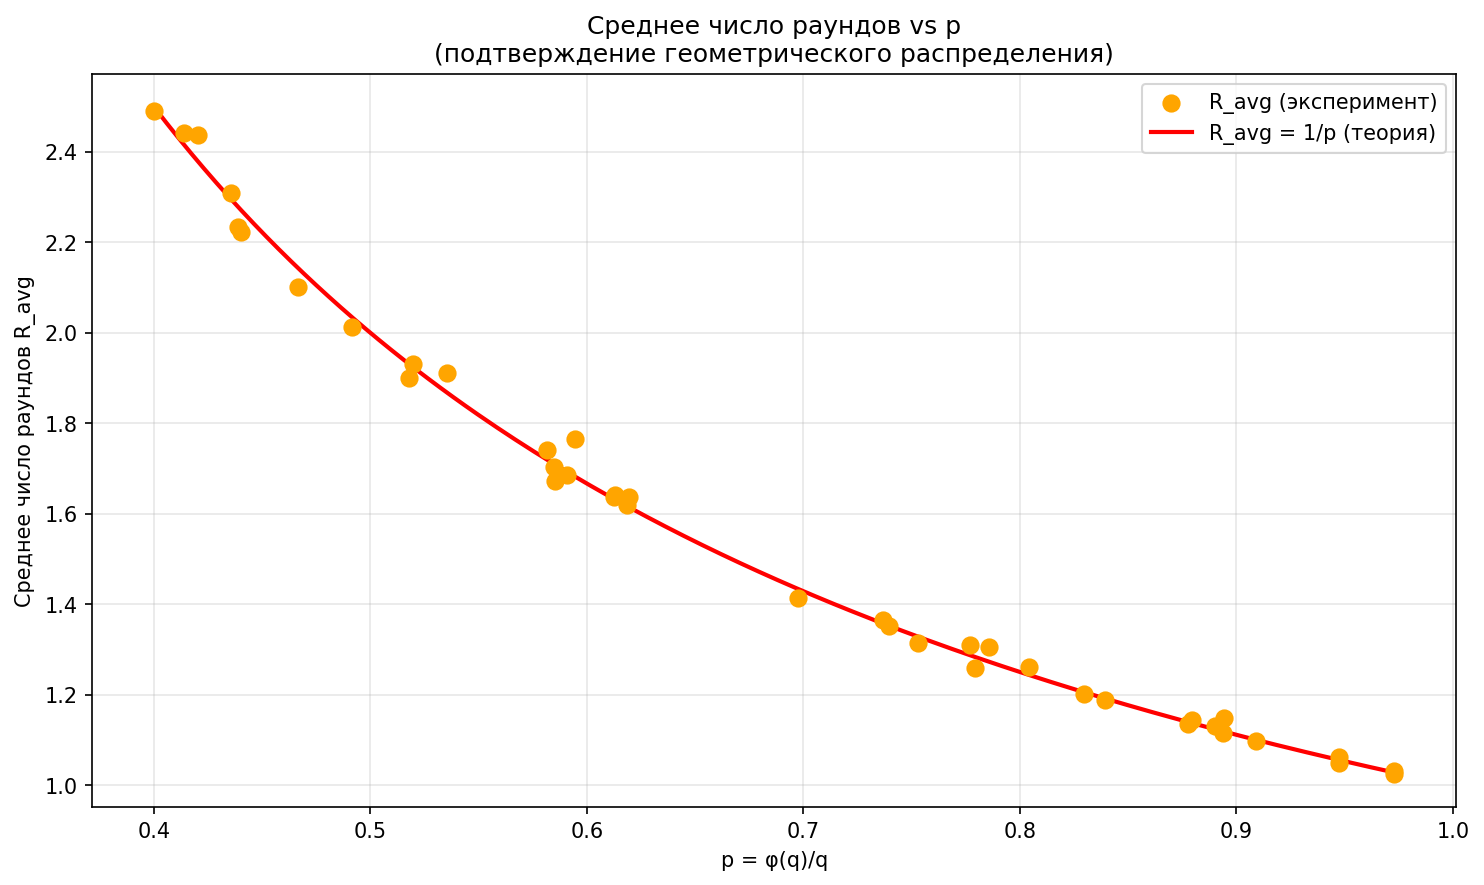
\includegraphics[width=1.15\textwidth]{image/2_2.png}}
    \caption{Зависимость среднего числа раундов от \(p\).}
\end{figure}

По формулам (1.9) – (1.11) вычислены \(R_{avg}\), \(R_{med}\), \(R_{mode}\), для каждой конфигурации. Для \(k = 1, p \approx 0.97: R_{avg} \approx 1.03\) раунда, \(R_{med} = 1\), \(R_{mode} = 1\). Теоретические значения: \(\frac{1}{p} \approx 1.03\), \(R_{med} = 1\), \(R_{mode} = 1\) — совпадают с экспериментальными.

На рисунке 2.2 показана зависимость среднего числа раундов \(R_{avg}\) от \(p\). По оси X — \(p = \frac{\phi(q)}{q}\) (от 0.40 до 0.97), по оси Y — \(R_{avg}\). Оранжевые точки — экспериментальные значения, красная кривая — теоретическая зависимость \(R_{avg} = \frac{1}{p}\).

\textbf{Оценка близости к теоретическому распределению}

\begin{figure}[H]
    \centering
    \makebox[\textwidth][c]{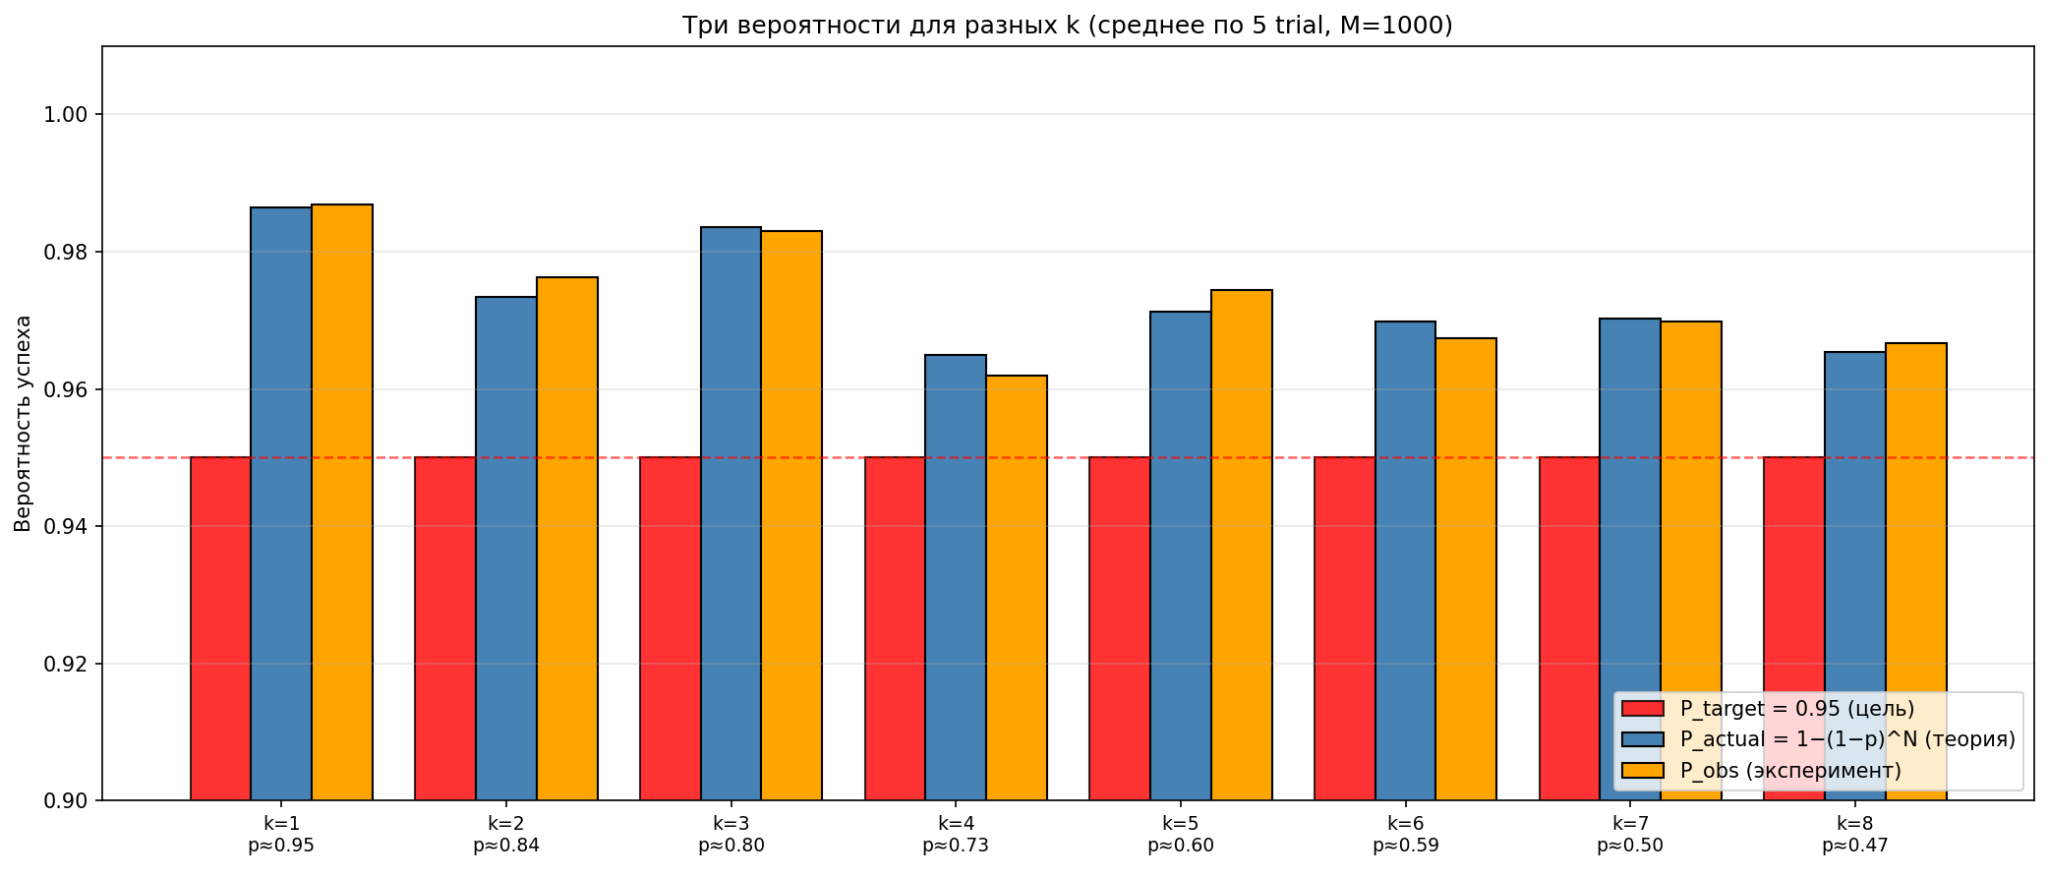
\includegraphics[width=1.15\textwidth]{image/2_3.png}}
    \caption{Оценка близости к теоретическому распределению}
\end{figure}

Сравненние целевой $P_{target}$, теоретической $P_{actual}$ и эксперементальной $P_{obs}$ вероятностей для $k \in \{ \overline{1.8} \}$ (среднее по 5 запускам). По оси $X$ — $k$ с указанием среднего $p$, по оси $Y$  — вероятность. Красные столбцы  — $P_{target} = 0.95$, синие — $P_{actual} = 1 - (1 - p)^N$, оранжевые  — $P_{obs} = \frac{a}{M}$.

Для всех $k$ значения $P_{actual}$ и  $P_{obs}$ совпадают с точностью до статистического разброса. Обе величины превышают $P_{target} = 0.95$ из-за дискретности $N$ округляется вверх, «перескакивая» через целевую вероятность.

\textbf{Проверка условия $\hat{P} \approx P$}

Условие методики $\hat{P} \approx P$ выполнено: расхождение $|P_{actual} - P_{obs}|$ не превышает 0.02, что в пределах $\pm 3 \sigma$ при $\sigma = \sqrt{\frac{P(1-P)}{M}} \approx 0.0069$.

Эксперементальное распределение числа раундов совпадает с теоретическим геометрическим параметром $p=\frac{\phi (q)}{q}$ при всех $k$.

Главные результат: вероятность успеха одна раунда $p=\frac{\phi (q)}{q}$ и среднее число раундов $R_{avg} \approx \frac{1}{p}$ зависят от структуры числа $q$ и величины простых делителей, но не от размера модуля $m$. Это подтверждено эксперементально на 40 конфигурациях с $p$ от 0.40 до 0.97.

\end{spacing}

\newpage
\section*{ЗАКЛЮЧЕНИЕ}
\addcontentsline{toc}{section}{ЗАКЛЮЧЕНИЕ}
\begin{spacing}{1.5} 
В ходе выполнения лабораторной работы был реализован вероятностный алгоритм поиска числа с заданным мультипликативным порядком по простому модулю с использованием теста простоты Соловея–Штрассена. Реализация выполнена на языке C++ с использованием библиотеки длинной целочисленной арифметики GMP. В соответствии с заданием, при реализации использовались только операции ввода-вывода, сложения, вычитания, сравнения, сдвига и побитовые операции; общее деление с остатком не применялось.

Было проведено экспериментальное исследование количества раундов алгоритма. Эксперимент показал, что количество раундов, необходимых для нахождения числа с заданным порядком, подчиняется геометрическому распределению с параметром \(p = \frac{\phi(q)}{q}\). Экспериментальные данные хорошо согласуются с теоретическими оценками: среднее число раундов \(R_{avg}\) с высокой точностью совпадает с теоретическим значением \(\frac{1}{p}\).

Анализ гистограмм распределения затрат для различных конфигураций \(q\) показал, что при увеличении числа простых делителей \(q\) (и, соответственно, уменьшении \(p\)) распределение становится более пологим, а математическое ожидание числа раундов возрастает. Полученные результаты подтверждают корректность реализации и справедливость вероятностных оценок, лежащих в основе алгоритма.
\end{spacing}

\newpage
\section*{СПИСОК ИСПОЛЬЗУЕМЫХ ИСТОЧНИКОВ}
\addcontentsline{toc}{section}{СПИСОК ИСПОЛЬЗУЕМЫХ ИСТОЧНИКОВ}
\begin{enumerate}
    \item Рыбин С.В. Дискретная математика и информатика : учебник для вузов. Санкт-Петербург: Лань, 2022.
    \item Solovay R., Strassen V. A fast Monte-Carlo test for primality // SIAM Journal on Computing. — 1977. — Vol. 6, No. 1. — P. 84–85.
\end{enumerate}

\newpage
\section*{ПРИЛОЖЕНИЕ А. Доказательства используемых утверждений}
\addcontentsline{toc}{section}{ПРИЛОЖЕНИЕ А. Доказательства используемых утверждений}

\begin{spacing}{1.5}

\noindent \textbf{Утверждение} (Совпадение значений функций Эйлера и функции Кармайкла).

\noindent Если \(m\) равно 2 или 4 или натуральной степени нечетного простого числа или удвоенной натуральной степени нечетного простого числа, то значения функции Эйлера и функции Кармайкла в точке \(m\) равны, т.е.
\[
    m \in (\{2, 4\} \cup P \cup (2P)) \Rightarrow \phi(m) = \lambda(m),
\]
где \(P = \{p^n \mid p \in \mathbb{P}'_{\mathbb{N}}, n \in \mathbb{N}\}\), \(\mathbb{P}'_{\mathbb{N}} = \mathbb{P}_{\mathbb{N}} \setminus \{2\}\).

\noindent Доказательство.
Рассмотрим все случаи:
\begin{enumerate}
    \item \(m = 2\): \(\phi(2) = 1, \lambda(2) = 1\). Равенство выполняется;
    \item \(m = 4\): \(\phi(4) = 2, \lambda(4) = 2\). Равенство выполняется;
    \item \(m = p^n\). Мультипликативная группа \(\mathbb{Z}_{p^n}^*\) является циклической.
    
    В циклической группе порядка \(\phi(p^n)\) существует элемент \(g\), порядок которого в точности равен размеру группы:
    \[
        P_{p^n}(g) = \phi(p^n)
    \]
    Отсюда \(\lambda(p^n) \ge P_{p^n}(g) = \phi(p^n)\), так как \(\lambda\) верхняя граница для порядков элементов.
    
    С другой стороны, для любого \(a\) взаимно простого с \(p^n\),
    \[
        a^{\phi(p^n)} \equiv 1 \pmod{p^n}.
    \]
    Следовательно
    \[
        \lambda(p^n) = \phi(p^n),
    \]
    ч.т.д.
\end{enumerate}

\vspace{1cm}

\noindent \textbf{Утверждение} (множество возможных значений показателя по модулю).

\noindent Множество возможных значений показателя по модулю \(m\) принадлежит натуральным делителям \(\lambda(m)\), т. е.
\[
    P_m(a) \in d(\lambda(m)),
\]
где \(a \perp m\).

\noindent Доказательство.
Так как
\[
    a^{\lambda(m)} \equiv 1 \pmod m,
\]
Разделим \(\lambda(m)\) на \(P_m(a)\) с остатком:
\[
    \lambda(m) = q \cdot P_m(a) + r, \quad 0 \le r < P_m(a).
\]
Рассмотрим \(a^r\)
\[
    r = \lambda(m) - q \cdot P_m(a)
\]
\[
    a^r = a^{\lambda(m) - q \cdot P_m(a)} = a^{\lambda(m)} \cdot (a^{P_m(a)})^{-q}
\]
\[
    a^r \equiv 1 \pmod m
\]
Предположим, что \(r > 0\). Тогда это означает, что \(P_m(a) \mid r\), что противоречит условию, ч.т.д.

\vspace{1cm}

\noindent \textbf{Утверждение} (мультипликативный порядок степени натурального числа):

\[
    \gamma = P_m(a) \Rightarrow P_m(a^b) = \frac{\gamma}{D(\gamma, b)},
\]
где \(D(\gamma, b)\) - наибольший общий делитель чисел \(\gamma\) и \(b\).

\noindent Доказательство.
Необходимо найти минимальное число \(k\) такое, чтобы
\[
    a^{bk} \equiv 1 \pmod m,
\]
то есть \(a^{bk} \equiv 1 \pmod m \Rightarrow \gamma \mid bk\). Тогда \(k = \frac{\gamma}{D(\gamma, b)}\) наименьшее натуральное число при котором это возможно, ч.т.д.

\vspace{1cm}

\noindent \textbf{Утверждение} (оценка сверху значения мультипликативного порядка):
\[
    a^{\frac{\lambda(m)}{q}} \not\equiv 1 \pmod m \Rightarrow P_m(a^{\frac{\lambda(m)}{q}}) \le q.
\]

\noindent Доказательство.
Обозначим \(x \equiv a^{\frac{\lambda(m)}{q}} \pmod m\). Возведем его в степень \(q\):
\[
    x^q \equiv a^{\lambda(m)} \equiv 1 \pmod m.
\]
Следовательно \(P_m(a^{\frac{\lambda(m)}{q}}) \le q\), ч.т.д.

\vspace{1cm}

\noindent \textbf{Утверждение} (тестирование числа на соответствие заданному мультипликативному порядку).

\noindent Пусть \(b = a^{\frac{\lambda(m)}{q}}\).
\[
    \forall e \in (d(q) \cap \mathbb{P}_N) \quad b^{\frac{q}{e}} \not\equiv 1 \pmod m \Rightarrow P_m(b) = q,
\]

\noindent Доказательство.
Обозначим \(r = P_m(b)\). Так как \(b^q \equiv 1 \pmod m\), то \(r \mid q\).
Пойдем от противного, пусть \(r < q\). Тогда число \(\frac{q}{r} > 1\) имеет простой делитель, обозначим его \(e\). Тогда
\[
    e \mid \frac{q}{r} \Rightarrow e \mid q.
\]
В таком случае
\[
    b^{\frac{q}{e}} \equiv (b^r)^{\frac{q}{r \cdot e}} \equiv 1 \pmod m,
\]
что противоречит условию, а значит \(r = q\), ч.т.д.

\vspace{1cm}

\noindent \textbf{Утверждение} (вероятность успеха при поиске числа с заданным показателем по простому модулю). При случайном выборе \(1 \le a \le m - 1\), где \(m\) - простое число, вероятность того, что \(b \equiv a^{\frac{m-1}{q}} \pmod m\) будет иметь показатель \(q\) по модулю \(m\), равно \(\frac{\phi(q)}{q}\).

\noindent Доказательство.
По теореме Гаусса существует \(g \in \{1, \dots, m-1\}\), такой что всякое \(a \in \{1, \dots, m-1\}\) единственным образом представимо в виде
\[
    a \equiv g^k \pmod m, \quad k \in \{0, \dots, m-2\}.
\]
При равновероятном выборе \(a\) показатель \(k\) равномерно распределен по \(\{0, \dots, m-2\}\).
Обозначим \(b \equiv a^{\frac{m-1}{q}} \pmod m\). Тогда
\[
    b \equiv g^{k \cdot \frac{m-1}{q}} \pmod m.
\]
Мультипликативный порядок степени равен
\[
    P_m(b) = \frac{m-1}{\gcd(m-1, k \cdot \frac{m-1}{q})}.
\]
Положим \(m-1 = qs\). Тогда
\[
    P_m(b) = \frac{qs}{\gcd(qs, ks)} = \frac{q}{\gcd(q, k)},
\]
Значит,
\[
    P_m(b) = q \Leftrightarrow \gcd(q, k) = 1.
\]
Остается посчитать долю таких \(k\).
Так как \(q \mid (m-1)\), на \(\{0, \dots, m-2\}\) укладывается ровно \(s = \frac{m-1}{q}\) полных периодов по модулю \(q\). В каждом периоде \(\phi(k)\) значений \(k\) взаимно простых с \(q\). Итого количество подходящих \(k\) равно
\[
    s \cdot \phi(q) = \frac{m-1}{q} \cdot \phi(q).
\]
В результате получается
\[
    Pr(P_m(b) = q) = \frac{\frac{m-1}{q} \cdot \phi(q)}{m-1} = \frac{\phi(q)}{q},
\]
ч.т.д.

\end{spacing}

\newpage
\section*{ПРИЛОЖЕНИЕ Б. Используемые функции}
\addcontentsline{toc}{section}{ПРИЛОЖЕНИЕ Б. Используемые функции}

\begin{spacing}{1.5}

\noindent Операции над \texttt{mpz\_class}, разрешенные к использованию:

\vspace{0.2cm}
\renewcommand{\arraystretch}{1.1} 
\noindent\begin{tabularx}{\textwidth}{|l|X|}
\hline
\textbf{Оператор} & \textbf{Назначение} \\
\hline
\texttt{a++} & Увеличивает значение a на единицу \\
\hline
\texttt{-a} & Возвращает число, противоположное значению a \\
\hline
\texttt{a + b} & Возвращает сумму значений a и b \\
\hline
\texttt{a - b} & Возвращает разность значений a и b \\
\hline
\texttt{a == b} & Возвращает \texttt{true}, если значения a и b равны, либо \texttt{false}, если значения a и b различны \\
\hline
\texttt{a != b} & Возвращает \texttt{true}, если значения a и b различны, либо \texttt{false}, если значения a и b равны \\
\hline
\texttt{a > b} & Возвращает \texttt{true}, если значение a больше значения b, иначе возвращает \texttt{false} \\
\hline
\texttt{a < b} & Возвращает \texttt{true}, если значение a меньше значения b, иначе возвращает \texttt{false} \\
\hline
\texttt{a | b} & Возвращает число, полученное при дизъюнкции соответствующих битов значений a и b \\
\hline
\texttt{a \& b} & Возвращает число, полученное при конъюнкции соответствующих битов значений a и b \\
\hline
\texttt{a << k} & Возвращает число, полученное сдвигом битов числа a влево на k позиций \\
\hline
\texttt{a >> k} & Возвращает число, полученное сдвигом битов числа a вправо на k позиций \\
\hline
\end{tabularx}

\vspace{0.5cm}

\noindent Используются нижеприведенные функции из заголовочного файла \texttt{<gmpxx.h>}.

\vspace{0.2cm}

\noindent\begin{tabularx}{\textwidth}{|X|}
\hline
\texttt{mpz\_class(const char* str)} \\
\hline
Конструктор. Создает длинное число из строки \\
\hline
\end{tabularx}

\vspace{0.2cm}

\noindent\begin{tabularx}{\textwidth}{|X|}
\hline
\texttt{gmp\_randclass(gmp\_randinit\_mt)} \\
\hline
Конструктор класса генератора псевдослучайных чисел. \\
\hline
\end{tabularx}

\vspace{0.2cm}

\noindent\begin{tabularx}{\textwidth}{|X|}
\hline
\texttt{void seed(unsigned long int seed)} \\
\hline
Метод класса \texttt{gmp\_randclass}. Инициализирует генератор псевдослучайных чисел значением seed. \\
\hline
\end{tabularx}

\vspace{0.2cm}

\noindent\begin{tabularx}{\textwidth}{|X|}
\hline
\texttt{mpz\_class get\_z\_range(const mpz\_class\& n)} \\
\hline
Метод класса \texttt{gmp\_randclass}. Возвращает случайное длинное число в диапазоне от 0 до n - 1 включительно \\
\hline
\end{tabularx}

\vspace{0.5cm}

\noindent Используются нижеприведенные функции из стандартной библиотеки C++ заголовочные файлы \texttt{<cmath>}, \texttt{<utility>}.

\vspace{0.2cm}

\noindent\begin{tabularx}{\textwidth}{|X|}
\hline
\texttt{abs(const mpz\_class\& a)} \\
\hline
Возвращает модуль (абсолютную величину) числа a. Для \texttt{mpz\_class} перегружена в \texttt{<gmpxx.h>} и возвращает новый объект \texttt{mpz\_class} \\
\hline
\end{tabularx}

\vspace{0.2cm}

\noindent\begin{tabularx}{\textwidth}{|X|}
\hline
\texttt{swap(mpz\_class\& a, mpz\_class\& b)} \\
\hline
Обменивает местами значения переменных a и b. Для \texttt{mpz\_class} имеет специализированную перегрузку в GMP. \\
\hline
\end{tabularx}

\vspace{0.5cm}

\noindent Используются нижеприведенные макросы и функции из заголовочного файла \texttt{<gtest/gtest.h>}, предназначенные для организации модульного тестирования.

\vspace{0.2cm}

\noindent\begin{tabularx}{\textwidth}{|X|}
\hline
\texttt{TEST(SuiteName, TestName)} \\
\hline
Объявляет тест без использования фикстуры. \\
\hline
\end{tabularx}

\vspace{0.2cm}

\noindent\begin{tabularx}{\textwidth}{|X|}
\hline
\texttt{TEST\_F(Fixture, TestName)} \\
\hline
Объявляет тест с использованием фикстуры \texttt{Fixture} (класса, унаследованного от \texttt{::testing::Test}. \\
\hline
\end{tabularx}

\vspace{0.2cm}

\noindent\begin{tabularx}{\textwidth}{|X|}
\hline
\texttt{EXPECT\_EQ(val1, val2)} \\
\hline
Проверяет, что значения val1 и val2 равны. При несовпадении выводит сообщение об ошибке и продолжает выполнение теста \\
\hline
\end{tabularx}

\vspace{0.2cm}

\noindent\begin{tabularx}{\textwidth}{|X|}
\hline
\texttt{EXPECT\_NE(val1, val2)} \\
\hline
Проверяет, что значения val1 и val2 не равны. \\
\hline
\end{tabularx}

\vspace{0.2cm}

\noindent\begin{tabularx}{\textwidth}{|X|}
\hline
\texttt{EXPECT\_GE(val1, val2)} \\
\hline
Проверяет, что значение val1 больше или равно val2 \\
\hline
\end{tabularx}

\vspace{0.2cm}

\noindent\begin{tabularx}{\textwidth}{|X|}
\hline
\texttt{EXPECT\_LT(val1, val2)} \\
\hline
Проверяет, что значение val1 строго меньше val2 \\
\hline
\end{tabularx}

\vspace{0.2cm}

\noindent\begin{tabularx}{\textwidth}{|X|}
\hline
\texttt{EXPECT\_THROW(statement, exception)} \\
\hline
Проверяет, что выполнение выражения \texttt{statement} выбрасывает исключение указанного типа \texttt{exception} \\
\hline
\end{tabularx}

\end{spacing}

\newpage
\section*{ПРИЛОЖЕНИЕ В. Разработанные функции}
\addcontentsline{toc}{section}{ПРИЛОЖЕНИЕ В. Разработанные функции}

\begin{spacing}{1.5}
\renewcommand{\arraystretch}{1.2}

\noindent\begin{tabularx}{\textwidth}{|X|}
\hline
\texttt{mpz\_class mul\_mod(const mpz\_class\& a, const mpz\_class\& b, const mpz\_class\& m)} \\
\hline
Вычисляет \(a \cdot b \pmod m\) \\
\hline
\end{tabularx}

\vspace{0.2cm}
\noindent\begin{tabularx}{\textwidth}{|X|}
\hline
\texttt{mpz\_class pow\_mod(const mpz\_class\& a, const mpz\_class\& b, const mpz\_class\& m)} \\
\hline
Вычисляет \(a^b \pmod m\) \\
\hline
\end{tabularx}

\vspace{0.2cm}
\noindent\begin{tabularx}{\textwidth}{|X|}
\hline
\texttt{mpz\_class gcd(const mpz\_class\& a, const mpz\_class\& b)} \\
\hline
Вычисляет наибольший общий делитель чисел \(a\) и \(b\) \\
\hline
\end{tabularx}

\vspace{0.2cm}
\noindent\begin{tabularx}{\textwidth}{|X|}
\hline
\texttt{mpz\_class find\_element\_with\_order(const mpz\_class\& q,}\\
\texttt{const std::vector<mpz\_class>\& qd, const mpz\_class\& m,}\\
\texttt{gmp\_randclass\& rng, int k)} \\
\hline
Вероятностный алгоритм поиска \(b\) такого, что \(P_m(b) = q\) \\
\hline
\end{tabularx}

\vspace{0.2cm}
\noindent\begin{tabularx}{\textwidth}{|X|}
\hline
\texttt{bool solovay\_strassen(const mpz\_class\& m, int k,}\\
\texttt{gmp\_randclass\& rng)} \\
\hline
Вероятностный тест простоты Соловея – Штрассена \\
\hline
\end{tabularx}

\vspace{0.2cm}
\noindent\begin{tabularx}{\textwidth}{|X|}
\hline
\texttt{mpz\_class jacobi(const mpz\_class\& a, const mpz\_class\& n)} \\
\hline
Вычисляет символ Якоби \(\left(\frac{a}{n}\right)\) итеративным бинарным алгоритмом, без деления с остатком. \\
\hline
\end{tabularx}

\vspace{0.5cm}
\noindent Функции, необходимые для тестирования исследуемого алгоритма.

\vspace{0.2cm}
\noindent\begin{tabularx}{\textwidth}{|X|}
\hline
\texttt{mpz\_class generate::prime(int bits, gmp\_randclass\& rng)} \\
\hline
Генерирует случайное простое число заданной битовой длины. Старший и младший биты принудительно устанавливаются в 1. Простота проверяется \\
\hline
\end{tabularx}

\vspace{0.2cm}
\noindent\begin{tabularx}{\textwidth}{|X|}
\hline
\texttt{mpz\_class generate::q\_from\_small\_primes(int k,}\\
\texttt{gmp\_randclass\& rng, std::vector<mpz\_class>\& qd\_out)} \\
\hline
Генерирует \(q\) как произведение \(k\) случайно выбранных простых из набора \(\{3, 5, 7, 11, \dots, 41\}\). Возвращает \(q\) и его простые делители. \\
\(k\) \hspace{0.8cm} — число простых в \(q\) \\
\(rng\) \hspace{0.5cm} — генератор псевдослучайных чисел \\
\(qd\_out\) — вектор простых делителей \(q\) \\
\hline
\end{tabularx}

\vspace{0.2cm}
\noindent\begin{tabularx}{\textwidth}{|X|}
\hline
\texttt{mpz\_class generate::m\_for\_q(const mpz\_class\& q, int}\\
\texttt{bits, gmp\_randclass\& rng, mpz\_class\& R\_out)} \\
\hline
Генерирует простое \(m = 2 \cdot q \cdot R + 1\), где \(R\) — простое. \\
Гарантирует \(q \mid m-1\) и известное разложение \(m-1 = 2 \cdot q \cdot R\). \\
\(q\) \hspace{0.8cm} — порядок, делитель \(m-1\) \\
\(bits\) \hspace{0.5cm} — битовая длина \(m\) \\
\(rng\) \hspace{0.5cm} — генератор псевдослучайных чисел \\
\(R\_out\) \hspace{0.2cm} — выходной параметр (простое \(R\)) \\
\hline
\end{tabularx}

\vspace{0.2cm}
\noindent\begin{tabularx}{\textwidth}{|X|}
\hline
\texttt{void assert\_valid\_order(const mpz\_class\& x, const}\\
\texttt{mpz\_class\& q, const std::vector<mpz\_class>\& qd, const}\\
\texttt{mpz\_class\& m)} \\
\hline
Проверяет, что \(x\) имеет порядок \(q\) по модулю \(m\) согласно свойству (1.7): \(x^q \equiv 1 \pmod m\), а для каждого простого делителя \(d \mid q\) выполняется \(x^{\frac{q}{d}} \not\equiv 1 \pmod m\). \\
Реализована через макросы \texttt{EXPECT\_*} фреймворка GoogleTest. \\
\hline
\end{tabularx}

\vspace{0.5cm}
\noindent Функции, необходимые для исследования алгоритма

\vspace{0.2cm}
\noindent\begin{tabularx}{\textwidth}{|X|}
\hline
\texttt{int runners::count\_N(const mpz\_class\& q, const}\\
\texttt{std::vector<mpz\_class>\& qd, double PTarget)} \\
\hline
Вычисляет минимальное число раундов N, при котором \(1 - (1 - p)^N > \texttt{PTarget}\), где \(p = \frac{\phi(q)}{q}\). \\
\(q\) \hspace{1.2cm} — заданный мультипликативный порядок \\
\(qd\) \hspace{1cm} — простые делители \(q\) \\
\(PTarget\) — целевая вероятность успеха \\
\hline
\end{tabularx}

\vspace{0.2cm}
\noindent\begin{tabularx}{\textwidth}{|X|}
\hline
\texttt{double runners::run\_find\_element\_with\_order(const}\\
\texttt{mpz\_class\& q, const std::vector<mpz\_class>\& qd, const}\\
\texttt{mpz\_class\& m, gmp\_randclass\& rng, double PTarget, int}\\
\texttt{l, std::vector<int>\& rounds\_out, int maxRounds)} \\
\hline
Запускает \texttt{find\_element\_with\_order} \(l\) раз с лимитом \texttt{maxRounds} раундов. Собирает номера раундов успешных запусков в \texttt{rounds\_out}, возвращает экспериментальную оценку \(P_{obs} = \frac{a}{M}\). \\
\(q\) \hspace{1.5cm} — порядок \\
\(qd\) \hspace{1.3cm} — простые делители \(q\) \\
\(m\) \hspace{1.4cm} — простой модуль \\
\(rng\) \hspace{1.2cm} — генератор псевдослучайных чисел \\
\(PTarget\) \hspace{0.4cm} — целевая вероятность (для вычисления \(N\_target\)) \\
\(l\) \hspace{1.6cm} — число запусков \(M\) \\
\(rounds\_out\) — номера раундов \(R\_i\) успешных запусков \\
\(maxRounds\) — лимит раундов на один запуск (\(N\_max\)) \\
\hline
\end{tabularx}

\vspace{0.2cm}
\noindent\begin{tabularx}{\textwidth}{|X|}
\hline
\texttt{int main() (в experiment.cpp)} \\
\hline
Точка входа эксперимента. Для \(k = 1..8\) и \(trials = 1..5\): \\
\hspace{0.5cm} генерирует \(q = \texttt{q\_from\_small\_primes}(k, rng, qd)\), \\
\hspace{0.5cm} генерирует \(m = \texttt{m\_for\_q}(q, 64, rng, R)\), \\
\hspace{0.5cm} вызывает \texttt{runners::run\_find\_element\_with\_order} c \(M = 1000\), \\
\hspace{0.5cm} сохраняет результаты в \texttt{summary.csv} и \texttt{rounds.csv}. \\
\hline
\end{tabularx}

\vspace{0.2cm}
\noindent\begin{tabularx}{\textwidth}{|X|}
\hline
\texttt{int main(int argc, char** argv) (в main.cpp)} \\
\hline
Демонстрация одного вызова \texttt{find\_element\_with\_order}. \\
Принимает из argv: \(m, q, qd[0], \dots, qd[n-1]\). \\
Проверяет, что \(m\) простое, \(q \mid m-1\), \(qd\) — простые делители \(q\) и выводит найденное \(x\) и номер раунда. \\
\hline
\end{tabularx}

\end{spacing}

\newpage
\section*{ПРИЛОЖЕНИЕ Г. Исходный код разработанной программы}
\addcontentsline{toc}{section}{ПРИЛОЖЕНИЕ Г. Исходный код разработанной программы}

\end{document}
